% Project 1 - EECS 499
% Authors: Shaun Howard and Matt Swartwout
\documentclass[conference]{IEEEtran} \usepackage[T1]{fontenc} \usepackage[backend=biber, style=ieee]{biblatex}
\addbibresource{report.bib} \usepackage[final]{microtype}

% *** GRAPHICS RELATED PACKAGES ***
%
\ifCLASSINFOpdf \usepackage[pdftex]{graphicx} % declare the path(s) where your graphic files are
  \graphicspath{{images/}} % and their extensions so you won't have to specify these with
  % every instance of \includegraphics
  \DeclareGraphicsExtensions{.jpeg,.png} \else % or other class option (dvipsone, dvipdf, if not using dvips). graphicx
  % will default to the driver specified in the system graphics.cfg if no
  % driver is specified.
  % \usepackage[dvips]{graphicx}
  % declare the path(s) where your graphic files are
  % \graphicspath{{../eps/}}
  % and their extensions so you won't have to specify these with
  % every instance of \includegraphics
  % \DeclareGraphicsExtensions{.eps}
\fi % graphicx was written by David Carlisle and Sebastian Rahtz. It is
% required if you want graphics, photos, etc. graphicx.sty is already
% installed on most LaTeX systems. The latest version and documentation
% can be obtained at:
% http://www.ctan.org/pkg/graphicx
% Another good source of documentation is "Using Imported Graphics in
% LaTeX2e" by Keith Reckdahl which can be found at:
% http://www.ctan.org/pkg/epslatex
%
% latex, and pdflatex in dvi mode, support graphics in encapsulated
% postscript (.eps) format. pdflatex in pdf mode supports graphics
% in .pdf, .jpeg, .png and .mps (metapost) formats. Users should ensure
% that all non-photo figures use a vector format (.eps, .pdf, .mps) and
% not a bitmapped formats (.jpeg, .png). The IEEE frowns on bitmapped formats
% which can result in "jaggedy"/blurry rendering of lines and letters as
% well as large increases in file sizes.
%
% You can find documentation about the pdfTeX application at:
% http://www.tug.org/applications/pdftex

% correct bad hyphenation here
\hyphenation{op-tical net-works semi-conduc-tor}


\begin{document}

% paper title
% Titles are generally capitalized except for words such as a, an, and, as,
% at, but, by, for, in, nor, of, on, or, the, to and up, which are usually
% not capitalized unless they are the first or last word of the title.
% Linebreaks \\ can be used within to get better formatting as desired.
% Do not put math or special symbols in the title.
\title{Distributed State Estimation in a 1-D World}


% author names and affiliations
% use a multiple column layout for up to three different
% affiliations
\author{ \IEEEauthorblockN{Shaun Howard \ \ Matt Swartwout} \IEEEauthorblockA{Electrical Engineering and Computer
Science Department\\ Case Western Reserve University\\ Cleveland, Ohio 44106\\ Email: \{smh150, mws85\}@case.edu} }

% make the title area
\maketitle

% As a general rule, do not put math, special symbols or citations
% in the abstract
\begin{abstract}
In this paper, we propose the use of both an Extended Kalman Filter (EKF) and an Unscented Kalman
Filter (UKF) in order to determine the x-position of a single mobile robot (R) given multiple noisy sensor measurements.
Given a squadron of N robots in a one-dimensional environment, the x-position of robot R with noisy odometry data can be
estimated via the sensor measurements of all N robots denoted S. Each robot in S can monitor the true position of R via
their laser scan sensor in order to build a set of pose estimates for R. The resulting set of N pose estimates can be
filtered in a distributed fashion either via an EKF or UKF in order to accurately estimate the current pose of R in the
one-dimensional environment.

We demonstrate the usefulness of this state estimation procedure through a three robot simulation in Gazebo. We compare
the results of the distributed filter with a self-filter in this environment where R estimates its own position via
object detection and either an EKF or UKF. We simulate the use of each filter with varying speeds of R. We analyze and
compare filter results from each simulation in order to determine the reliability of each filter. Our simulation results
reveal that the distributed filter frequently out-performs the self-filter in terms of accuracy without any additional
parameter tuning.
\end{abstract}

% Same thing here, we didn't actually look into attacking any sensors
The idea behind the method is derived from the method proposed in [1]. Their method uses an EKF to predict the position
of one terrorized robot given N sensor measurements. The difference between the methods is that this method analyses the
usage of an EKF as well as UKF for estimating the position of a terrorized robot given N-1 measurements from remote
sensors and a single sensor measurement given point cloud data from the affected robot. Both filters show remarkable
results in tracking the terrorized robot's position over time, but the UKF beats the EKF in accuracy most of the time.
The simulation uses three robots with one terrorized and monitored by the other two to test the estimation hypothesis
and prove that UKF works with one-dimensional robot position estimation from N noisy sensor measurements.

\section{Introduction} \label{Introduction}
Networked cyber-physical systems have become more and more common in recent history. Traditionally, as the need for more
accuracy and precision has evolved with these systems the response has been to add more sensors. These sensors, when
combined together, e.g. a Kalman filter, can provide better state estimation than a single sensor alone. This is also
significantly cheaper than developing single sensors with extraordinary accuracy. However, as mobile robots and other
mobile autonomous technologies become more widespread the desire to decrease the cost and complexity of these devices
has increased. Adding more and more sensors to a single robot, while effective, is not cost-efficient for production and
leads to higher maintenance costs over the life of the robot.

One solution to this is distributed sensor networks. With recent developments in high-bandwith mobile radio
communications, sharing large amounts of sensor data over wireless networks has become much more feasible. Instead of
putting many sensors on one robot, many robots can use their one sensor and their observations of the other robots
around them to create a distributed state estimate for their companions.

Our system is based on the TurtleBot 2 platform and the Robot Operating System (ROS) \cite{ros_original}. The system is a simple 1-Dimensional exploration of the feasibility of distributed state estimation, using a mobile robot and two stationary landmarks as shown in \ref{pic1}. The mobile robot, using a LIDAR distance sensor, determines its position in the world by comparing itself to known stationary landmarks. At the same time, the known landmarks also use LIDAR to determine the mobile robots position. All of this data is then fused together in a Kalman filter, and compared to the output of a Kalman filter of just the robot's individual sensor, and also the ground truth of the simulator. Our simulations compare not only the "self" and "distributed" versions of the filter, but also examine the Extended Kalman Filter vs Unscented Kalman Filter and how they respond differently to the configurations. We also simulate the robot's motion at different speeds and compare the filter's performance when that is modified.

\begin{figure}[!ht]
\label{pic1} 
\centering 
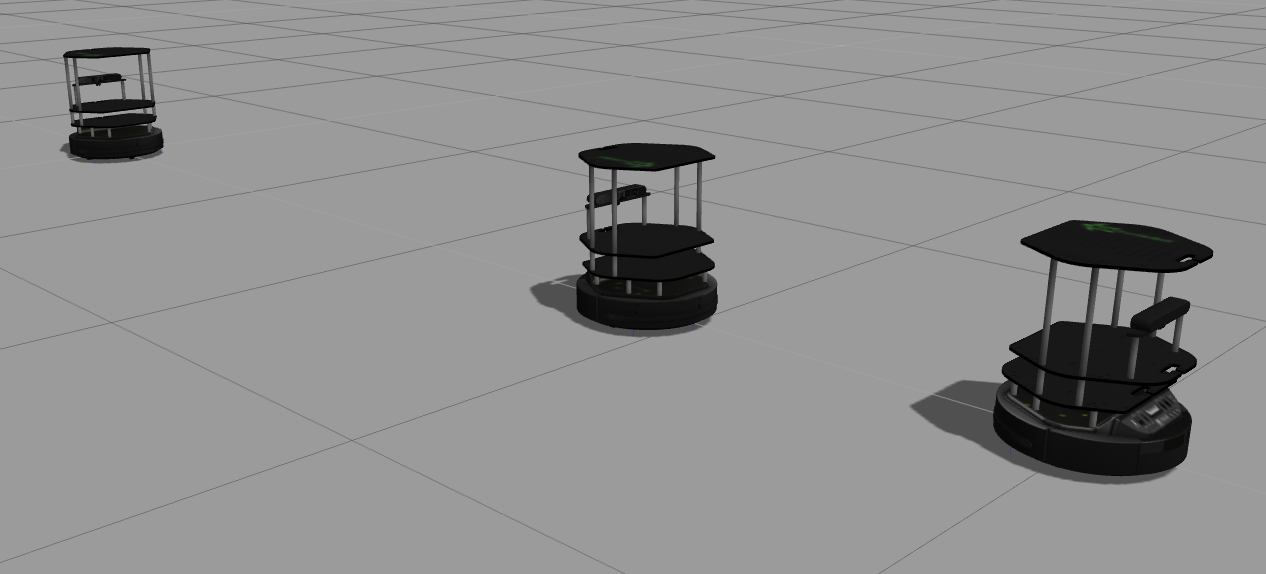
\includegraphics[scale=.2]{sim1}
\caption{Three TurtleBots on a world-based grid world attempt to estimate the position of the moving robot.}
\end{figure}

There are two primary contributions of this paper. First, we outline a system in ROS that implements a distributed sensor network between three robots, and is easily scalable to an arbitrary number. Second, we compare the performance of different filters in both the distributed and egocentric world-view.

\subsection{Related Work}

\section{Problem Formulation} \label{Problem Formulation} % This should probably go in the introduction somewhere
The concept of sensor fusion and combining multiple sensor readings within a single robot has been well shown. By
combining data from multiple sensors and feeding that information into an EKF or UKF, the total accuracy of the system
can be improved. Inherent noise in one sensor will propagate less into the final result, and the loss of a single or
multiple sensors will not necessarily result in catastrophic failure of the system.

Our problem specification is created from these core tenets:
\begin{enumerate} 
\item A finite 1-D system containing a mobile robot 
\item A physical landmark (e.g. stationary robot) at each end of the system \item The mobile robot and
landmarks are all equipped with a sensor that measures distance \item The mobile robot can move forwards and backwards,
but cannot change its orientation (this obviates the need for a recognition system between the robot and landmarks)
\end{enumerate}

The core problems solved in the implementation of this system are:
\begin{enumerate} \item Implementation of Extended and Unscented Kalman filters via the robot\_localization package \cite{robot_localization}
\item Create a ROS system that simulates a TurtleBot 2 and the stationary landmarks in Gazebo \cite{gazebo}.
\item Create a ROS node system for the TurtleBot 2 that facilitates communication between the mobile robot and the stationary landmarks, and also
transforms and feeds those measurements into the filters. 
\end{enumerate} 

\section{Methodology} \label{Methodology} As stated above, the project naturally divided itself into three main
problems. These three problems were the implementation of the Extended and Unscented Kalman filters, simulation of the
TurtleBot 2 and 1-D environment in Gazebo, and creating the system of ROS nodes for the TurtleBot 2 to communicate with
the stationary landmarks and the filters.

\subsection{Sensor Measurements} \label{Sensor Measurements} Before describing our filter, we will describe how we
collected our distance measurements. Our measurements were taken by a simulated Microsoft Kinect camera, v1.0. We used
the depthimage\_to\_laserscan package \cite{depth_to_scan} to create a simulated LIDAR. Every scan (of ROS type
sensor\_msgs/LaserScan) received included a large number of ranges from different points in the scan. We used this
collection of ranges to create a single scan point that we then fed into the filter. We found that taking the median of
the scan ranges was far more accurate than the mean, so each filter input was the median of the scan ranges, with the
variance of the measurement being the variance of the entire group of measurements that was taken.

\subsection{Filter Implementation} \label{Filter Implementation} We chose to implement our filters using the previously
mentioned robot\_localization. We chose this package due to its ability to do sensor fusion of an arbitrary number of
sensors, because it was built for ROS, and because of the simple setup but also the complex configurations that it
enables.

We implemented both an Extended and Unscented Kalman filter, but the actual configuration parameters for both of them
were identical. Additionally, we implemented two filters on the mobile robot. The first we called the "Self" filter, and
used only one distance measurements, taken by the robot's distance sensor to the landmark directly in front of it. The
second filter we called the "Distributed" filter, and it took measurements from the robot's sensor, and also both of the
landmark's sensors. All measurements were fed to the filter as a geometry\_msgs/PoseWithCovarianceStamped messages.

For both filters we set two\_d\_mode to true, because we did not care about any 3-dimensional motion. For the first
sensor measurement, we fused the x and y position and yaw into the final state estimate. Even though we assume a 1-D
system with no y movement possible, and also assume that no yaw rotations will ever be made, the filters do not support
a 1-D world so we had to include the y and yaw measurements. For the second and third sensor on the Distributed filter,
we fused only the x position.

We also set the differential parameter to true for all sensors. This makes the filter differentiate the absolute
position measurements received and input them as velocities rather than positions. This had two distinct advantages for
our system. First, we did not need to worry about transforming the poses from the reference frame of the landmark to the
reference frame of the mobile robot. Since we knew the starting position of the robot we did not need the absolute
position measurements. Second, this reduced the error from our measurement system. The system we used was a Kinect
camera, and we took a slice of points from its depth cloud and used this to simulate a LIDAR. Because of this, we were
not measuring a specific, known point on the robot. Instead, we measured many points and then took the median of those
points and represented that as the distance to the robot. By using the velocities rather than positions we mitigated
some of the error that may have come from the median point of the scan on the robot being in slightly different
positions from scan to scan. While error there may have existed, it would not lead to discrete jumps like the position
measurement would have.

We did not utilize any of the advanced parameters for either filter, and for the Unscented Kalman Filter we left the
alpha, beta, and kappa values at their defaults (0.001, 0, and 2, respectively). Once running, the filter nodes
published their topics via the standard ros publish/subscribe system and we were able to view this data.


\subsection{Gazebo Simulation} \label{Gazebo Simulation} Our simulation experiments were run in Gazebo with three
robots, two at fixed positions (stationary landmarks) and one moving randomly between the two (mobile robot). During
each experiment, the mobile robot moved randomly in the x-direction at a chosen experimental speed. Two speeds of 0.2
m/s and 0.4 m/s were chosen during experimentation for each filter type in order to determine the performance of filters
at various speeds in the one-dimensional environment.

The robot models used were the default TurtleBot 2 URDFs provided by the TurtleBot ROS package \cite{turtlebot}. The
robots were spawned into the world following the instructions laid out in the Gazebo Bringup Guide, with each robot
brought up inside of its own namespace to avoid conflicts.

The robots were spawned at Gazebo world coordinate (0,0), (2,0), and (4,0). The random motion of the mobile robot was
allowed between (1,0), and (3,0). These limits were chosen based on the Kinect's maximum range of 4m and minimum range
of .8m. To create the random motion, the robot would get a random number between -1 and 1 from a uniform distribution
and use that as an amount to move, with negative being backwards and positive forwards. Then a check was done to see if
the final position after the move wo uld be inside the movement bounds. If not, a new movement amount was generated. If
the move was acceptable, it was executed, with the progress being monitored by the Gazebo generated odometry. This
random motion repeated infinitely until stopped.

\subsection{Inter-Node Communication System} \label{Inter-Node Communication System} The communication system between
the ROS nodes was created very simply using the ros publish/suscribe paradigm. Each of the TurtleBots constantly
processed the received LaserScans, as outlined in \ref{Sensor Measurements} and published them to a topic call
processed\_scan. The mobile robot then subscribed to these topics and created Pose readings based on that sensor
measurement. These Pose readings were then published on their own topic, which the filters were configured to subscribe
too. Finally, the filters output their total state estimation reading on a separate topic, which we were then able to
record, graph, etc.

In essence, the use of ROS greatly simplified the networking of this system. Rather than having to work through the
intricacies of networking the robots together, we were able to create a system that is extensible to an arbitrary number
of robots and extremely resilient to failures, while also being incredibly simple.

\section{Results} \label{Results} % discuss and display sim vs filtered odom using std dev error bars
\subsection{Data Acquisition and Analysis} \label{Data Acquisition and Analysis}
The ros topics odometry pose messages echoed are 
recorded during the experiment with rosbag, converted to comma-separated value files, and analysed statistically with 
python and numpy. We visualize the results using matplotlib with a Matlab plotting interface via python. If one of the 
captured odometry topics is sampled at a higher frequency, a moving window average is used to estimate the data to match 
the other measurements one-to-one for analysis purposes. We take several statistics from the odometry data gathered per each experiment. 

\subsection{EKF Experiments} \label{EKF Experiments}
\subsubsection{R at 0.2 m/s} \label{R at 0.2 m/s}
The first experiment runs the simulation with R moving at 0.2 m/s. Figure 2 shows a table of the result statistics for experiment 1 - EKF 
with R at 0.2 m/s. 

%\begin{figure}[!ht]
%\label{pic2} 
%\centering 
%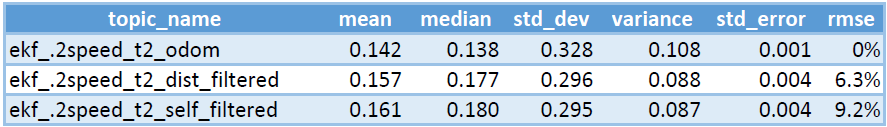
\includegraphics[scale=.2]{ekf_.2_table}
%\end{figure}

The data shows that the standard deviation, error and variance is higher in the distributed filter measurements than the 
self-filter measurements, but the self-filter has a higher root mean squared-error in accordance with the actual simulator odometry measurements than the distributed filter. From this fact, we can estimate that the distributed filter will perform better in this experiment than the self-filter. 

Figure 3 displays a comparison of the predicted odometry measurements via the self EKF to the actual simulator 
odometry. As depicted in the image, the self filter is not always within one standard deviation of the exact simulator 
odometry value. The self EKF tends to be inaccurate with sharp direction changes but is more reliable over time along a smooth interval.

\begin{figure}[!ht]
\label{pic3} 
\centering 
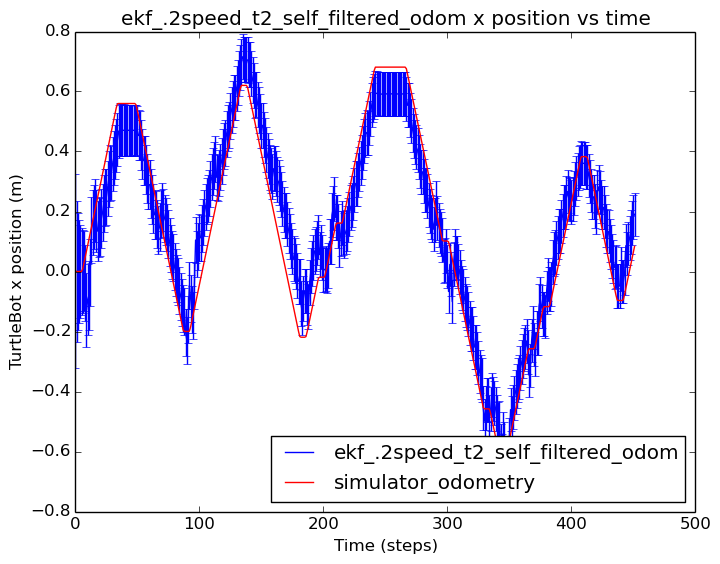
\includegraphics[scale=.45]{ekf_2speed_t2_self_filtered_odom_pos_err_graph}
\caption {A plot of the self-EKF position estimate along the simulator odometry curve over time 
reveals the inaccuracies of the ego-centric EKF along sharp changes in direction.}
\end{figure}

\par
Figure 4 displays a comparison between the distributed EKF filter with R at 0.2 m/s and simulator odometry. The 
distributed filter tends to be within one standard deviation of the actual odometry values according to the graph. 
Given the tolerable error on position estimation in the distributed EKF, it clearly outperforms the self-filter 
in this experiment. Looking at the graph, we observe that the distributed filter handles sharp changes in direction well, and the simulator odometry measurement is always within one standard deviation from the filter estimate.

\begin{figure}[!ht]
\label{pic4} 
\centering 
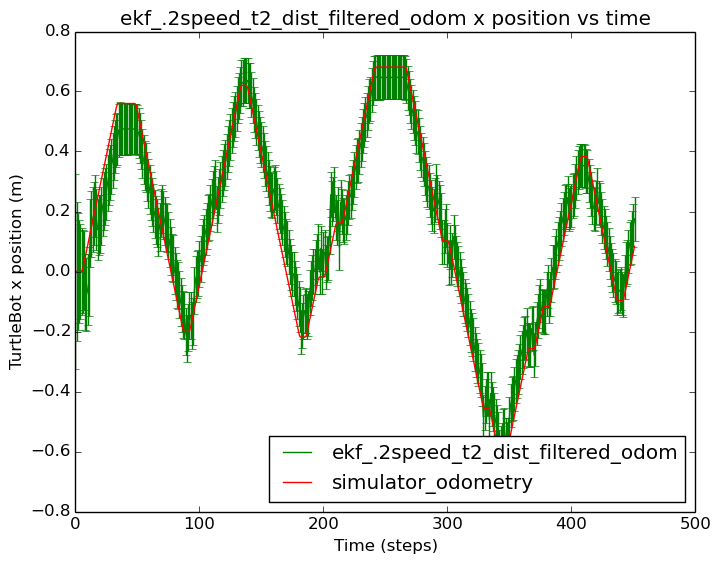
\includegraphics[scale=.45]{ekf_2speed_t2_dist_filtered_odom_pos_err_graph}
\caption {A plot of the distributed-EKF position estimate along the simulator odometry curve over time. It 
reveals the enhanced accuracy of the distributed filter over the ego-centric EKF. The distributed filter does not suffer 
from the inaccuracies in sharp direction changes that the self-filter does.}
\end{figure}

\subsubsection{R at 0.4 m/s} \label{R at 0.4 m/s}
The second experiment runs the simulation with R moving at 0.4 m/s. Figure 5 shows a table of the result statistics for 
experiment 2 - EKF with R at 0.4 m/s. 

%\begin{figure}[!ht]
%\label{pic5} 
%\centering 
%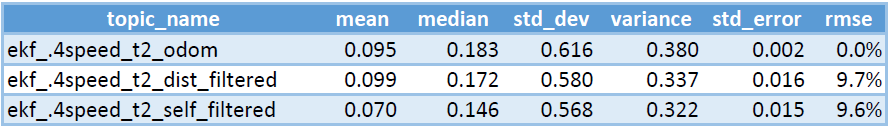
\includegraphics[scale=.2]{ekf_.4_table}
%\end{figure}

The statistics reveal that the self-filter has a lower variance, standard deviation and error than the distributed 
filter. However, the mean and median of the distributed filter position estimates closely agree with the mean of the 
simulator odometry measurements. This hints that the self-filter is more precise with estimate generation, but it is 
still less reliable than the distributed filter at estimating position in all one-dimensional movement scenarios.

Figure 6 displays a comparison of the predicted odometry measurements via the self EKF to the actual simulator 
odometry. As depicted in figure 3, the self filter is not always within one standard deviation of the exact simulator 
odometry value. The inaccuracies in the self-filter are upheld in addition to a erroneous drift that is corrected over 
time.

\begin{figure}[!ht]
\label{pic6} 
\centering 
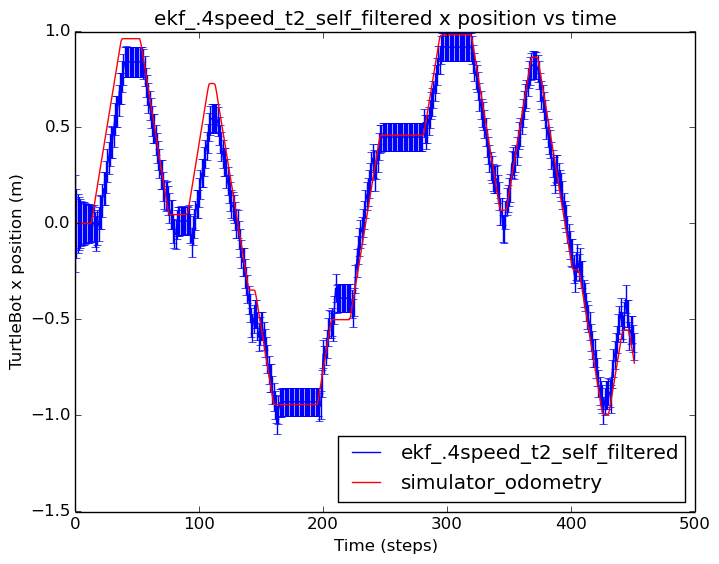
\includegraphics[scale=.45]{ekf_4speed_t2_self_filtered_pos_err_graph}
\caption {A second plot of the self-EKF position estimate along the simulator odometry curve over time 
upholds the inaccuracies of the ego-centric EKF in response to sudden changes in movement.}
\end{figure}

Figure 7 graphs the distributed EKF along the simulator odometry curve. The measurements are usually within one standard 
deviation of the actual values, but they reveal the inaccurate nature of the EKF with sudden changes in movement. These 
sudden changes tend to create a brief drift that flows through the system until it is shortly corrected. The support of 
the hypothesis in reference to the accuracy of the distributed EKF is slowly growing.

\begin{figure}[!ht]
\label{pic7} 
\centering 
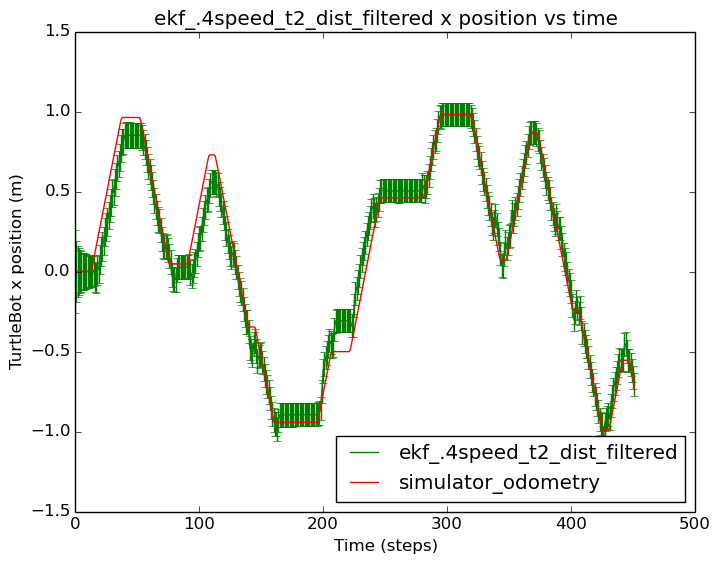
\includegraphics[scale=.45]{ekf_4speed_t2_dist_filtered_pos_err_graph}
\caption {A second plot of the distributed EKF position estimate along the simulator odometry curve over time 
upholds that the distributed EKF is usually more accurate than the self-filter but can also be prone to drift on sudden 
perturbations.}
\end{figure}

As we can see, the distributed EKF is prone to drift via sudden perturbations in movement like the self-EKF but 
eventually corrects itself in little time. The rate at which it corrects itself is quicker than that of the self-filter. 
This is most likely due to the confidence the system has in the three sensor measurements over that it has in the single 
sensor measurement from R. However, this figure shows more uncertainty at a higher speed than figure 4. Perhaps some 
modifications to the EKF -- the UKF -- will facilitate our proof of the hypothesis.

\subsection{UKF Experiments} \label{UKF Experiments}
\subsubsection{R at 0.2 m/s} \label{R at 0.2 m/s}
The third experiment runs the simulation with R moving at 0.2 m/s. Figure 8 shows a table of the result statistics for experiment 3 - UKF 
with R at 0.2 m/s. 

%\begin{figure}[!ht]
%\label{pic8} 
%\centering 
%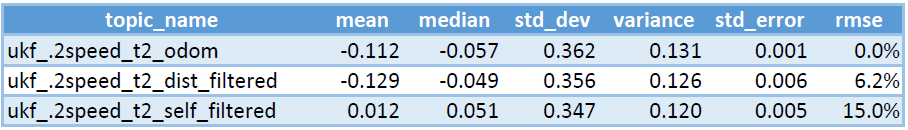
\includegraphics[scale=.2]{ukf_.2_table}
%\end{figure}

The data consistently shows that the standard deviation, error and variance are higher by a small amount in 
the distributed filter measurements when compared with the self-filter measurements as with the EKF. However, 
the self-filter still has a higher root mean squared-error in accordance with the actual simulator odometry 
measurements than the distributed filter. From this fact, we can estimate that the distributed filter will 
again perform better in this experiment than the self-filter.

Figure 9 displays the self UKF filter at work with R at 0.2 m/s randomly moving back 
and forth. The results of the run are not as favorable as previously seen. The 
errors may be due to random ros sensor errors or lack of parameter tuning. Perhaps 
the distributed UKF will perform better as predicted.

\begin{figure}[!ht]
\label{pic9} 
\centering 
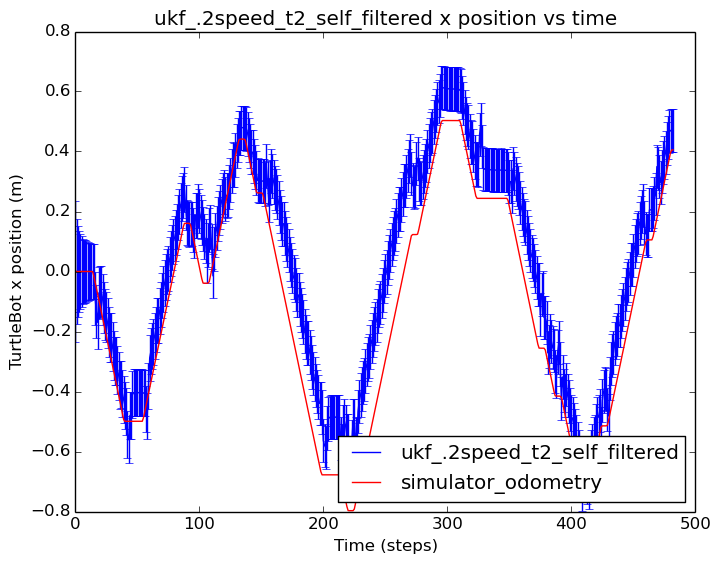
\includegraphics[scale=.45]{ukf_2speed_t2_self_filtered_pos_err_graph}
\caption {A plot of the self-UKF position estimate along the simulator odometry curve over time.}
\end{figure}

The distributed UKF performs well in its experiment, as predicted. The self-filter 
is consistently more inaccurate than the distributed filter so far. One more 
experiment should be able to conclude the simulation process. Figure 10 graphs the 
experiment. 

\begin{figure}[!ht]
\label{pic10} 
\centering 
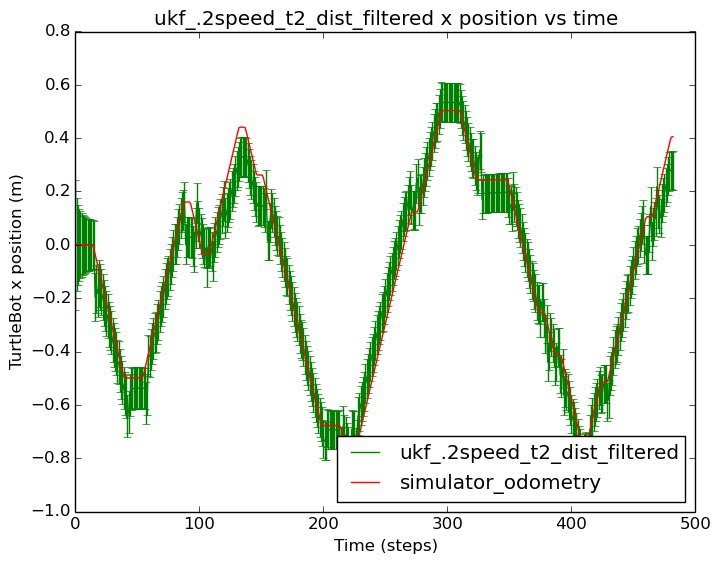
\includegraphics[scale=.45]{ukf_2speed_t2_dist_filtered_pos_err_graph}
\caption {A plot of the distributed UKF position estimate along the simulator odometry curve over time.}
\end{figure}


Figure 11 displays the results of running the self UKF at 0.4 m/s. The UKF does not 
appear to be very reliable for a single measurement at a higher speed. The measurements 
sometimes drift far off course and take a while to converge back to a reasonable 
confidence interval.

\begin{figure}[!ht]
\label{pic11} 
\centering 
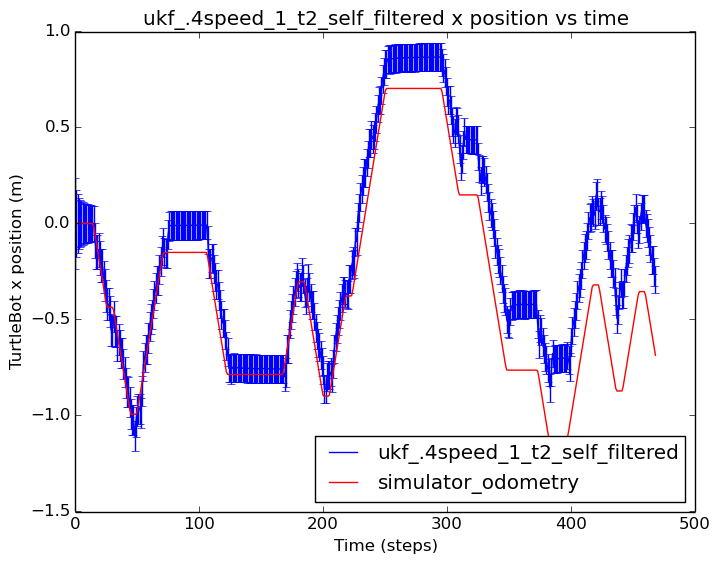
\includegraphics[scale=.45]{ukf_4speed_1_t2_self_filtered_pos_err_graph}
\caption {A second plot of the self-UKF position estimate along the simulator 
odometry curve over time.}
\end{figure}

Here we see that the self-UKF is no good for even a one-dimensional world with the default parameters.
The distributed UKF in figure 12 unsurprisingly reveals that more sensor measurements lead to a greater
precision and recall in the filter as compared to the self-filter. 

\begin{figure}[!ht]
\label{pic12} 
\centering 
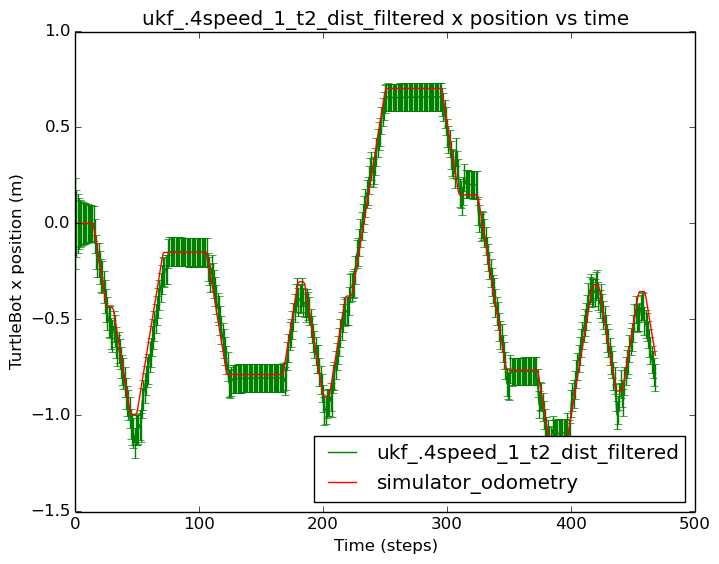
\includegraphics[scale=.45]{ukf_4speed_1_t2_dist_filtered_pos_err_graph}
\caption {A second plot of the distributed UKF position estimate along the simulator 
odometry curve over time.}
\end{figure}

Comparing both filtering approaches, we observe that the distributed filter almost always out-performs the self-filter 
with both filter types. Additionally, by no surprise we find that the UKF distributed filtering method out-performs the EKF distributed
filtering method. Overall, the results of our simulation support our hypothesis about the application of an EKF or UKF to accurately
estimate the position of a single mobile robot R via N sensor measurements given N robots networked in a distributed fashion in a 1-D environment. 
The self and distributed EKF work moderately well, but the UKF only works well with default parameters in a distributed system set up of at least 
two robots. Given more samples, the system was able to filter the data more accurately. We have shown that both the EKF and UKF work well in a 
distributed set up. Hopefully the idea of networking robots to share and predict accurate positional and state information will break new ground in 
the world of distributed and intelligent robotics network systems as a whole.

\section{Conclusion} \label{Conclusion} 
The conclusion goes here.

\section*{Acknowledgement}

The authors would like to thank...

\printbibliography

\end{document}
